\section{Per-coordinate statistics are set by the Gram matrix}
\label{app:per-coordinate}

An earlier version of this work summarised the stage-3 trajectories with statistics of
individual feature coordinates: how often a coordinate changes sign between consecutive
blocks, how much of its travel does not contribute to its net displacement and how
often it reverses twice or more.
Such statistics depend on the feature basis, which is not privileged: a rotation of the
channels that is absorbed by the adjacent linear layers leaves the network's function
unchanged and changes them.
This appendix shows that, for these trajectories, they are almost entirely determined
by the Gram matrix $G$ of the block increments, so they carry no information beyond the
basis-independent statistics of \cref{sec:coherence}.

\paragraph{Statistics.}
For each image, with the massive channel removed, write $\Delta x_{k,i}$ for the change
of coordinate $i$ over the unit interval $[k,k{+}1]$ and
$\mathrm{net}_i=\sum_k\Delta x_{k,i}$.
\emph{Excess travel} is $1-\sum_i|\mathrm{net}_i|/\sum_{k,i}|\Delta x_{k,i}|$;
the \emph{monotone share} is the mass-weighted share of coordinates whose nine
increments all have the same sign;
the \emph{sign-change rate} is the share of consecutive pairs $(k,k{+}1)$ with opposite
signs;
the \emph{reversed mass} adds $\min(|\Delta x_{k,i}|,|\Delta x_{k+1,i}|)$ over those
pairs, normalised by $\sum_{k,i}|\Delta x_{k,i}|$;
and the \emph{repeated sign-change share} is the mass-weighted share of coordinates that
change sign at least twice.
All statistics use every coordinate; the earlier text described a selection of the
coordinates whose net displacement is above the per-image median, but the code applied
it only to the median $t_{50}$ of the per-coordinate progress.

\paragraph{Surrogates.}
We replace the real increments by two surrogates that keep $G$ and discard everything
else: Gaussian increments with the same Gram matrix, and the real increments after a
random orthogonal rotation of the channels (three seeds each).
\Cref{tab:app-per-coordinate} shows that both reproduce every statistic within $0.03$
on the untied stage (at $R{=}1$ and $R{=}100$) and within $0.08$ on the tied one.
Tied coordinates are slightly more monotone than their surrogates, the only
basis-dependent structure we find.
A sign-change rate of $0.45$ is thus what a consecutive cosine of $0.17$ implies in any
basis, and the random stage, at cosine $0$, has a higher one.
Per spatial position the picture is the same: the cosine between consecutive untied
increments restricted to one position has a 10th percentile of $0.03$ at $R{=}1$, and
no position has a cosine below $-0.3$.

\begin{table}[t]
    \centering
    \caption{Per-coordinate statistics of stage~3 at integer times ($R{=}100$, $500$
    images, massive channel removed) for the real increments and for Gaussian
    increments with the same Gram matrix (mean over three seeds; std $\le 0.001$).}
    \label{tab:app-per-coordinate}
    \scriptsize
    \setlength{\tabcolsep}{2.5pt}
    \resizebox{\linewidth}{!}{%
    \begin{tabular}{llrrrrr}
        \toprule
        Stage & source & excess & monotone & sign change & reversed & repeated \\
        \midrule
        Random ($g^\ast$) & real      & 0.671 & 0.046 & 0.500 & 0.294 & 0.966 \\
        Untied            & real      & 0.477 & 0.230 & 0.446 & 0.249 & 0.902 \\
        Untied            & same Gram & 0.490 & 0.205 & 0.445 & 0.262 & 0.905 \\
        Tied              & real      & 0.188 & 0.739 & 0.114 & 0.018 & 0.137 \\
        Tied              & same Gram & 0.215 & 0.689 & 0.123 & 0.020 & 0.153 \\
        \bottomrule
    \end{tabular}%
    }
\end{table}

\paragraph{Gaussian prediction.}
If two increments are jointly Gaussian across coordinates with correlation $c$, a
coordinate changes sign with probability $\arccos(c)/\pi$.
With the measured consecutive cosine, this predicts a sign-change rate of $0.447$ for
the untied stage at $R{=}1$, against $0.447$ measured, and $0.217$ for the tied stage,
against $0.183$ measured; the prediction and the measurement correlate at $0.92$ to
$0.96$ across images and block pairs, and random blocks give $0.500$.

\paragraph{A nuance on the rotation argument.}
A literal channel-wise rotation absorbed by the adjacent linear layers would leave the
network's function unchanged and would change the per-coordinate statistics.
ConvNeXt is not quite that object: the depthwise convolution, the per-channel
LayerScale and the gains of LayerNorm all act per channel, and the massive activation
shows that the channel basis is partly privileged
(\cref{app:massive-activations}).
The empirical result nevertheless stands: Gaussian and randomly rotated surrogates that
keep $G$ reproduce the per-coordinate statistics to the tolerances above, so those
statistics add nothing beyond the Gram geometry of \cref{sec:coherence}.

\paragraph{Pooled coordinates.}
\Cref{fig:pooled-dynamics} shows the per-coordinate progress
$p_i(t)=(x_i(t)-x_i(0))/\mathrm{net}_i$ pooled over images.
The tied coordinates advance mostly monotonically, while the untied ones change course
at block boundaries: across one boundary $44.6\%$ of the coordinates of the velocity
change sign, against $0.19\%$ per micro-step inside a block.
By the argument above, this is the per-coordinate trace of nearly orthogonal increments,
not evidence that later blocks remove earlier ones; \cref{sec:coherence}
shows that they do not.
Script: \texttt{scripts/undo\_geometry\_audit.py}; outputs in
\texttt{outputs/undo\_audit}.

\begin{figure*}[t]
    \centering
    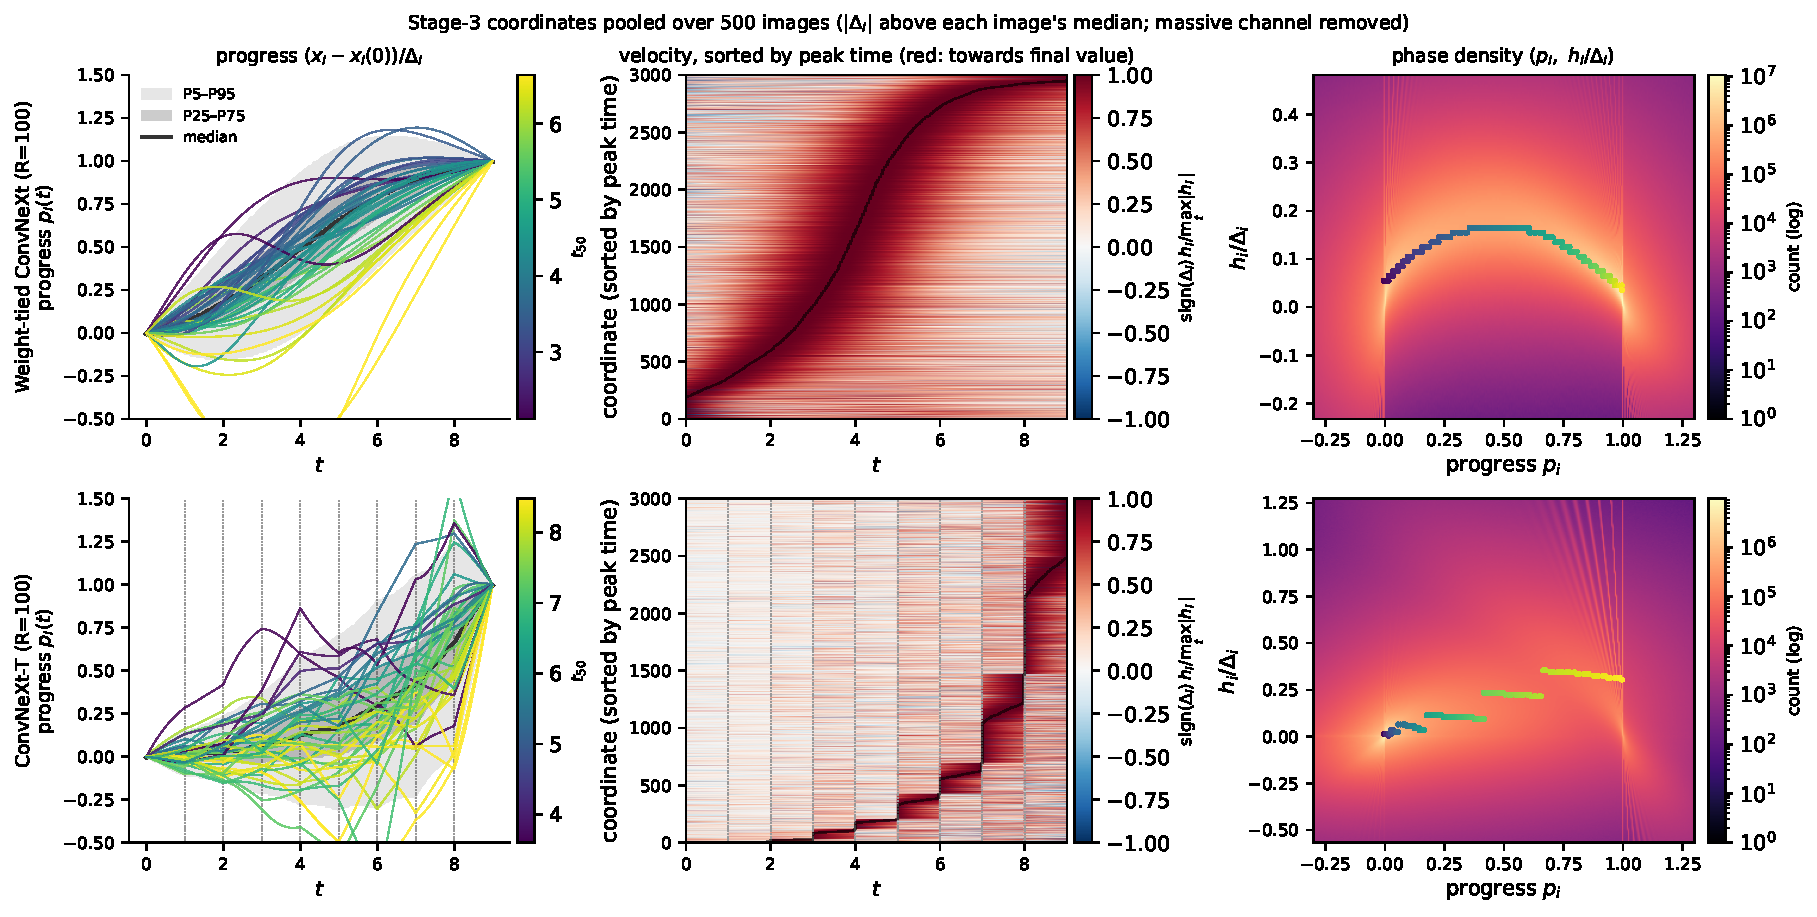
\includegraphics[width=\textwidth]{figures/pooled_dynamics.pdf}
    \caption{Stage-3 coordinates pooled over $500$ images ($R{=}100$; massive channel
    removed).
    \textbf{Top:} weight-tied ConvNeXt; \textbf{bottom:} untied ConvNeXt-T.
    \textbf{Left:} per-coordinate progress $p_i(t)$ (median and P5--P95; thin lines:
    random coordinates).
    \textbf{Middle:} velocity toward the final value, coordinates sorted by peak time
    (red: toward the end state; blue: away).
    \textbf{Right:} phase density $(p_i,\,h_i/\mathrm{net}_i)$.}
    \label{fig:pooled-dynamics}
\end{figure*}
